\documentclass{beamer}
\usefonttheme[onlymath]{serif}
\usepackage{geometry}
\usepackage[main=russian,english]{babel}
\usepackage[utf8]{inputenc}
\usepackage[T2A]{fontenc}
\usepackage{graphicx}
\usepackage[backend=bibtex,style=numeric, defernumbers=true]{biblatex}
% =======================================================
\usepackage{tikz}
\usetikzlibrary{shadows,arrows}
\usetikzlibrary{shapes.geometric,positioning,calc,shapes.misc}
\usepackage{pgfplots, pgfplotstable}
\usepgfplotslibrary{fillbetween}
\usepackage{tikz-dependency}
\usepackage{verbatim}
\usepackage[normalem]{ulem}
% =======================================================
\usepackage{algorithm2e}
% =======================================================
\usepackage{pdfpages}

\hypersetup{
pdfauthor={Лемтюжникова Д.В, Кудинов И.Д},
pdftitle={Кореференция в научно-техническом русском языке},
pdfsubject={d},
pdfkeywords={Кореференция, обработка текста, лингвистика, машинное обучение},
pdfproducer={d}
}

\usepackage{amsmath, amsthm, amssymb, amsfonts, cancel}
\usepackage{ifthen, titlesec, mathtext, enumerate, float, makeidx, bm}
\usepackage{verbatim, wrapfig, physics, floatflt, capt-of}

\usepackage{pgfplots, tikz}
\usetikzlibrary{positioning}

\usepackage{tikz-dependency}

\usepackage{color}
\usepackage{xcolor}
\definecolor{Mycolor1}{HTML}{5044d4}
\definecolor{Mycolor2}{HTML}{736ad9}
\definecolor{Mycolor3}{HTML}{8d86d9}
\definecolor{Mycolor4}{HTML}{8e4fe0}
\definecolor{MyGray}{HTML}{808080}
\newcommand{\tri}{{\color{blue!40} $\blacktriangleright$}\:}
\newcommand\mybox[2][]{\tikz[overlay]\node[fill=blue!20,inner sep=1pt, anchor=text, rectangle, rounded corners=1mm,#1] {#2};\phantom{#2}}

\graphicspath{{img/}}

\pgfplotsset{width = 6cm}

% \usepackage{pgfplots}

\addbibresource{/home/ilja/Documents/TeX/Диплом/Article1/Cites/sources.bib}


\usepackage[normalem]{ulem}

\makeatother
\makeindex
\usetheme{boxes}
\usecolortheme{seahorse}

\title{Разрешение проблемы кореференции}
\author{}
\date{}

% =======================================================
\tikzstyle{layer_base}=[rectangle,line width=2pt,minimum size=20pt,inner sep=0pt]

\tikzstyle{layer_gray}=[layer_base,draw=gray,fill=gray!20]
\tikzstyle{layer_red}=[layer_base,draw=red,fill=red!20]
\tikzstyle{layer_green}=[layer_base,draw=green,fill=green!20]
\tikzstyle{layer_blue}=[layer_base,draw=blue,fill=blue!20]
\tikzstyle{layer_yellow}=[layer_base,draw=yellow,fill=yellow!20]
\tikzstyle{layer_orange}=[layer_base,draw=orange,fill=orange!20]

\tikzstyle{neuron}=[circle,line width=1pt,draw=black,fill=white,minimum size=14pt,inner sep=0pt]
\tikzstyle{neuron_s}=[line width=1pt,draw=black!60,fill=white,minimum size=14pt,inner sep=0pt,xshift=-3ex]

\tikzstyle{normalvec}=[->, line width=1pt]
% =======================================================

\SetStartEndCondition{ }{}{}%
\SetKwProg{Fn}{def}{\string:}{}
\SetKwFunction{Range}{range}%%
\SetKw{KwTo}{in}\SetKwFor{For}{for}{\string:}{}%
\SetKwIF{If}{ElseIf}{Else}{if}{:}{elif}{else:}{}%
\SetKwFor{While}{while}{:}{fintq}%
\AlgoDontDisplayBlockMarkers\SetAlgoNoEnd\SetAlgoNoLine%


\begin{document}

\begin{frame}{CSG-геометрия}
\footnotesize

\tri Браш это выпуклый многогранник. Геометрия мира формируется из брашей вручную:

\begin{center}
\scalebox{0.65}{
\begin{tikzpicture}
    \filldraw [layer_gray] (0, 0) rectangle (0.5, 2);
    \filldraw [layer_gray] (0, 2) rectangle (5, 2.5);
    \filldraw [layer_gray] (4.5, 2) rectangle (5, -2);
    \filldraw [layer_gray] (2, 0) rectangle (2.5, -2);
    \filldraw [layer_gray] (0, -0.5) rectangle (2, 0);
    \filldraw [layer_gray] (2, -2) rectangle (5, -2.5);
    \filldraw [layer_gray] (3.75, 1.25) rectangle (4.5, 2);
    
    \node[font=\fontsize{40}{0}\selectfont] at (6, 0) {$\to$};
    
    \filldraw [layer_gray, draw=white] (7 + 0, -2.5) rectangle (7 + 5, 2.5);
    \coordinate (p1) at (7 + 0.5, 0);
    \coordinate (p2) at (7 + 0.5, 2);
    \coordinate (p3) at (7 + 3.75, 2);
    \coordinate (p4) at (7 + 3.75, 1.25);
    \coordinate (p5) at (7 + 4.5, 1.25);
    \coordinate (p6) at (7 + 4.5, -2);
    \coordinate (p7) at (7 + 2, -2);
    \coordinate (p8) at (7 + 2, 0);
    \draw[fill=white, line width=2pt, draw=green!60!black] (p1) -- (p2) -- (p3) -- (p4) -- (p5) -- (p6) -- (p7) -- (p8) -- cycle;
\end{tikzpicture}
}
\end{center}

\tri Карта, составленная из брашей, имеет слишком много полигонов. Задача CSG-алгоритма -- перевести множество брашей в замкнутую поверхность из полигонов. Игровой мир находится внутри этой поверхности, за ней находится заполненное пространство.

\end{frame}





\begin{frame}{CSG-геометрия: объединение двух брашей}
\footnotesize

\tri Пусть нужно объединить браши $A$ и $B$:
\begin{center}
\scalebox{0.45}{
\begin{tikzpicture}
    \filldraw [layer_gray] (0, 0) rectangle (2, 2);
    \filldraw [layer_gray] (1.5, 1.5) rectangle (3.5, 3.5);
    \filldraw [layer_gray,fill=none] (0, 0) rectangle (2, 2);
    \filldraw [layer_gray,fill=none] (1.5, 1.5) rectangle (3.5, 3.5);
    \node[font=\fontsize{20}{0}\selectfont] () at (1, 1) {$A$};
    \node[font=\fontsize{20}{0}\selectfont] () at (2.5, 2.5) {$B$};
    
    \node[font=\fontsize{40}{0}\selectfont] at (4.75, 1.75) {$\to$};
    
    \coordinate (p1) at (6 + 0, 0);
    \coordinate (p2) at (6 + 0, 2);
    \coordinate (p3) at (6 + 1.5, 2);
    \coordinate (p4) at (6 + 1.5, 3.5);
    \coordinate (p5) at (6 + 3.5, 3.5);
    \coordinate (p6) at (6 + 3.5, 1.5);
    \coordinate (p7) at (6 + 2, 1.5);
    \coordinate (p8) at (6 + 2, 0);
    \draw[layer_gray, draw=green!60!black] (p1) -- (p2) -- (p3) -- (p4) -- (p5) -- (p6) -- (p7) -- (p8) -- cycle;
    \node[font=\fontsize{20}{0}\selectfont] () at (6 + 1, 1) {$A'$};
    \node[font=\fontsize{20}{0}\selectfont] () at (6 + 2.5, 2.5) {$B'$};
\end{tikzpicture}
}
\end{center}
Сопоставим $A$ с $B$, получив набор полигонов $A'$:
\begin{center}
\scalebox{0.45}{
\begin{tikzpicture}
    \filldraw [layer_gray, draw=green!60!black] (0, 0) rectangle (2, 2);
    \filldraw [layer_gray] (1.5, 1.5) rectangle (3.5, 3.5);
    \node[font=\fontsize{20}{0}\selectfont] () at (1, 1) {$A$};
    \node[font=\fontsize{20}{0}\selectfont] () at (2.5, 2.5) {$B$};
    
    \node[font=\fontsize{40}{0}\selectfont] at (4.75, 1.75) {$\to$};
    
    \filldraw [layer_gray, fill=white, draw=green!60!black] (6 + 0, 0) rectangle (6 + 2, 2);
    \filldraw [fill=white, draw=white] (6 + 1.5, 1.5) rectangle (6 + 3.5, 3.5);
    \node[font=\fontsize{20}{0}\selectfont] () at (6 + 1, 1) {$A'$};
\end{tikzpicture}
}
\end{center}
Сопоставим $B$ с $A$, получив набор полигонов $B'$:
\begin{center}
\scalebox{0.45}{
\begin{tikzpicture}
    \filldraw [layer_gray, draw=green!60!black] (1.5, 1.5) rectangle (3.5, 3.5);
    \filldraw [layer_gray] (0, 0) rectangle (2, 2);
    \node[font=\fontsize{20}{0}\selectfont] () at (1, 1) {$A$};
    \node[font=\fontsize{20}{0}\selectfont] () at (2.5, 2.5) {$B$};
    
    \node[font=\fontsize{40}{0}\selectfont] at (4.75, 1.75) {$\to$};
    
    \filldraw [layer_gray, fill=white, draw=green!60!black] (6 + 1.5, 1.5) rectangle (6 + 3.5, 3.5);
    \filldraw [fill=white, draw=white] (6 + 0, 0) rectangle (6 + 2, 2);
    \node[font=\fontsize{20}{0}\selectfont] () at (6 + 2.5, 2.5) {$B'$};
\end{tikzpicture}
}
\end{center}
Объединяем $A'$ и $B'$, получаем результат.
\end{frame}





\begin{frame}{CSG-геометрия: объединение брашей уровня}
\footnotesize

\tri Для компиляции уровня из списка брашей необходимо сопоставить каждый браш с каждым:
\begin{center}
    \begin{algorithm}[H]
    \SetKwFunction{FMain}{csgCompile}
    \Fn{\FMain{$brushes$}}{
        $brushesCopy \leftarrow \mathrm{copy}(brushes)$\;
        \For{$A' \in brush$}{
            \For{$B \in brushesCopy ~\backslash~ A$}{
                $A' \leftarrow \mathrm{clip}(A', B)$\;
            }
        }
    }
    \end{algorithm}
\end{center}

\tri В итоге $brushes$ будет хранить итоговый набор полигонов уровня.

\end{frame}





\begin{frame}{CSG-геометрия: разрез браша брашем}
\footnotesize

\tri В функции $\mathrm{clip}$ из каждого полигона $b1$ необходимо вырезать ту часть что находится внутри $b2$. Переберём полигоны $A'$: берём левый полигон $A'$ -- он находится вне $B$ и не пересекается с ним -- игнорировать:
\begin{center}
\scalebox{0.4}{
\begin{tikzpicture}
    \filldraw [layer_gray] (0, 0) rectangle (2, 2);
    \filldraw [layer_gray] (1.5, -1) rectangle (3.5, 3);
    \filldraw [layer_gray,fill=none] (0, 0) rectangle (2, 2);
    \filldraw [layer_gray,fill=none] (1.5, -1) rectangle (3.5, 3);
    \node[font=\fontsize{20}{0}\selectfont] () at (1, 1) {$A'$};
    \node[font=\fontsize{20}{0}\selectfont] () at (2.5, 1) {$B$};
        \draw[draw=red, line width=2pt] (0, 0) -- (0, 2);
    
    \node[font=\fontsize{40}{0}\selectfont] at (4.75, 1) {$\to$};
        
    \filldraw [layer_gray] (6 + 0, 0) rectangle (6 + 2, 2);
    \filldraw [layer_gray] (6 + 1.5, -1) rectangle (6 + 3.5, 3);
    \filldraw [layer_gray,fill=none] (6 + 0, 0) rectangle (6 + 2, 2);
    \filldraw [layer_gray,fill=none] (6 + 1.5, -1) rectangle (6 + 3.5, 3);
    \node[font=\fontsize{20}{0}\selectfont] () at (6 + 1, 1) {$A'$};
    \node[font=\fontsize{20}{0}\selectfont] () at (6 + 2.5, 1) {$B$};
        \draw[draw=green!60!black, line width=2pt] (6 + 0, 0) -- (6 + 0, 2);
\end{tikzpicture}
}
\end{center}
Берём верхний полигон $A'$, он пересекается полигонами из $B$ -- разрезать и отбросить правую часть:
\begin{center}
\scalebox{0.4}{
\begin{tikzpicture}
    \filldraw [layer_gray] (0, 0) rectangle (2, 2);
    \filldraw [layer_gray] (1.5, -1) rectangle (3.5, 3);
    \filldraw [layer_gray,fill=none] (0, 0) rectangle (2, 2);
    \filldraw [layer_gray,fill=none] (1.5, -1) rectangle (3.5, 3);
    \node[font=\fontsize{20}{0}\selectfont] () at (1, 1) {$A'$};
    \node[font=\fontsize{20}{0}\selectfont] () at (2.5, 1) {$B$};
        \draw[draw=green!60!black, line width=2pt] (0, 0) -- (0, 2);
        \draw[draw=red, line width=2pt] (0, 2) -- (2, 2);
    
    \node[font=\fontsize{40}{0}\selectfont] at (4.75, 1) {$\to$};
        
    \filldraw [layer_gray] (6 + 0, 0) rectangle (6 + 2, 2);
    \filldraw [layer_gray] (6 + 1.5, -1) rectangle (6 + 3.5, 3);
    \filldraw [layer_gray,fill=none] (6 + 0, 0) rectangle (6 + 2, 2);
    \filldraw [layer_gray,fill=none] (6 + 1.5, -1) rectangle (6 + 3.5, 3);
    \node[font=\fontsize{20}{0}\selectfont] () at (6 + 1, 1) {$A'$};
    \node[font=\fontsize{20}{0}\selectfont] () at (6 + 2.5, 1) {$B$};
        \draw[draw=green!60!black, line width=2pt] (6 + 0, 0) -- (6 + 0, 2);
        \draw[draw=green!60!black, line width=2pt] (6 + 0, 2) -- (6 + 1.5, 2);
        \draw[draw=gray!20, line width=2pt] (6 + 1.55, 2) -- (6 + 2.1, 2);
\end{tikzpicture}
}
\end{center}
Берём правый полигон $A'$, он полностью внутри $B$ -- удалить:
\begin{center}
\scalebox{0.4}{
\begin{tikzpicture}
    \filldraw [layer_gray] (0, 0) rectangle (2, 2);
    \filldraw [layer_gray] (1.5, -1) rectangle (3.5, 3);
    \filldraw [layer_gray,fill=none] (0, 0) rectangle (2, 2);
    \filldraw [layer_gray,fill=none] (1.5, -1) rectangle (3.5, 3);
    \node[font=\fontsize{20}{0}\selectfont] () at (1, 1) {$A'$};
    \node[font=\fontsize{20}{0}\selectfont] () at (2.5, 1) {$B$};
        \draw[draw=green!60!black, line width=2pt] (0, 0) -- (0, 2);
        \draw[draw=green!60!black, line width=2pt] (0, 2) -- (1.5, 2);
        \draw[draw=gray!20, line width=2pt] (1.55, 2) -- (2.1, 2);
        \draw[draw=red, line width=2pt] (2, 2) -- (2, 0);
    
    \node[font=\fontsize{40}{0}\selectfont] at (4.75, 1) {$\to$};
        
    \filldraw [layer_gray] (6 + 0, 0) rectangle (6 + 2, 2);
    \filldraw [layer_gray] (6 + 1.5, -1) rectangle (6 + 3.5, 3);
    \filldraw [layer_gray,fill=none] (6 + 0, 0) rectangle (6 + 2, 2);
    \filldraw [layer_gray,fill=none] (6 + 1.5, -1) rectangle (6 + 3.5, 3);
    \node[font=\fontsize{20}{0}\selectfont] () at (6 + 1, 1) {$A'$};
    \node[font=\fontsize{20}{0}\selectfont] () at (6 + 2.5, 1) {$B$};
        \draw[draw=green!60!black, line width=2pt] (6 + 0, 0) -- (6 + 0, 2);
        \draw[draw=green!60!black, line width=2pt] (6 + 0, 2) -- (6 + 1.5, 2);
        \draw[draw=gray!20, line width=2pt] (6 + 1.55, 2) -- (6 + 2.1, 2);
        \draw[draw=gray!20, line width=2pt] (6 + 2, 2) -- (6 + 2, 0);
\end{tikzpicture}
}
\end{center}

\end{frame}





\begin{frame}{CSG-геометрия: разрез браша брашем}
\footnotesize

\tri В итоге получаем $A'$:
\begin{center}
\scalebox{0.4}{
\begin{tikzpicture}
    \filldraw [layer_gray, draw=green!60!black] (0, 0) rectangle (2, 2);
    \filldraw [layer_gray] (1.5, -1) rectangle (3.5, 3);
    \node[font=\fontsize{20}{0}\selectfont] () at (1, 1) {$A'$};
    \node[font=\fontsize{20}{0}\selectfont] () at (2.5, 1) {$B$};
\end{tikzpicture}
}
\end{center}

\tri В случае сечения $B'$ при помощи $A$ все стороны сохранятся кроме левой: она будет разрезана на три части, центральная из которых удалится поскольку находится внутри $A$:
\begin{center}
\scalebox{0.4}{
\begin{tikzpicture}
    \filldraw [layer_gray, draw=green!60!black] (1.5, -1) rectangle (3.5, 3);
    \filldraw [layer_gray] (0, 0) rectangle (2, 2);
    \node[font=\fontsize{20}{0}\selectfont] () at (1, 1) {$A$};
    \node[font=\fontsize{20}{0}\selectfont] () at (2.5, 1) {$B'$};
        \draw[draw=red, line width=2pt] (1.5, 0) -- (1.5, 2);
\end{tikzpicture}
}
\end{center}

\tri Псевдокод $\mathrm{clip}$ выглядит так:
\begin{center}
    \begin{algorithm}[H]
    \SetKwFunction{FMain}{csgCompile}
    \Fn{\FMain{$A', ~ B$}}{
        $newPolygonList \leftarrow {}[]$\;
        \For{$p \in A'.polygons$}{
            $\mathrm{clipPolygon}(A'.polygons, p, B)$\:
        }
        \KwRet{$newPolygonList$}
    }
    \end{algorithm}
\end{center}

\end{frame}





\begin{frame}{CSG-геометрия: разрез полигона брашем}
\footnotesize

\tri Функция разреза полигона $p$ набором полигонов $B$ работает так: определяется положение $p$ относительно $B$:
\begin{enumerate}
    \item Если $p$ находится снаружи $B$, то $p$ возвращается в не изменённом виде (рис 1.);
    \item Если $p$ находится внутри $B$, то ничего не возвращать (рис 2.);
    \item Если $p$ лежит на $q$, одном из полигонов $B$, и их нормали совпадают, вернуть один из них чтобы не образовалось дыры, а другой полигон будет рассечён позже (рис 3.). Обычно возвращают полигон того браша, который сечётся позже;
    \item Если три предыдущих проверки не прошли, $p$ точно пересекается одним или несколькими полигонами $L \subseteq B.polygons$ браша $B$.
\end{enumerate}

\begin{center}
\scalebox{0.4}{
\begin{tikzpicture}
    \filldraw [layer_gray] (0, 0) rectangle (2, 2);
    \filldraw [layer_gray] (1.5, -1) rectangle (3.5, 3);
    \filldraw [layer_gray,fill=none] (0, 0) rectangle (2, 2);
    \filldraw [layer_gray,fill=none] (1.5, -1) rectangle (3.5, 3);
    \node[font=\fontsize{20}{0}\selectfont] () at (1, 1) {$A'$};
    \node[font=\fontsize{20}{0}\selectfont] () at (2.5, 1) {$B$};
        \draw[draw=red, line width=2pt] (0, 0) -- (0, 2);
        
        \node[font=\fontsize{20}{0}\selectfont] () at (1.75, -2) {$1.$};
\end{tikzpicture}
}~~~
\scalebox{0.4}{
\begin{tikzpicture}
    \filldraw [layer_gray] (0, 0) rectangle (2, 2);
    \filldraw [layer_gray] (1.5, -1) rectangle (3.5, 3);
    \filldraw [layer_gray,fill=none] (0, 0) rectangle (2, 2);
    \filldraw [layer_gray,fill=none] (1.5, -1) rectangle (3.5, 3);
    \node[font=\fontsize{20}{0}\selectfont] () at (1, 1) {$A'$};
    \node[font=\fontsize{20}{0}\selectfont] () at (2.5, 1) {$B$};
        \draw[draw=red, line width=2pt] (2, 0) -- (2, 2);
        
        \node[font=\fontsize{20}{0}\selectfont] () at (1.75, -2) {$2.$};
\end{tikzpicture}
}~~~
\scalebox{0.4}{
\begin{tikzpicture}
    \filldraw [layer_gray] (0, 0) rectangle (2, 2);
    \filldraw [layer_gray] (0, -1) rectangle (3.5, 3);
    \filldraw [layer_gray,fill=none] (0, 0) rectangle (2, 2);
    \filldraw [layer_gray,fill=none] (0, -1) rectangle (3.5, 3);
    \node[font=\fontsize{20}{0}\selectfont] () at (1, 1) {$A'$};
    \node[font=\fontsize{20}{0}\selectfont] () at (2.5, 1) {$B$};
        \draw[draw=red, line width=2pt] (0, 0) -- (0, 2);
        \draw[normalvec, line width=3pt] (0, 1) -- (-1, 1);
        \draw[normalvec, draw=red, line width=3pt] (0, 1) -- (-0.5, 1);
        
        \node[font=\fontsize{20}{0}\selectfont] () at (1.75, -2) {$3.$};
\end{tikzpicture}
}
\end{center}

\end{frame}





\begin{frame}{CSG-геометрия: относительное положения точки}
\footnotesize

\begin{center}
\begin{minipage}{0.65\textwidth}
    \tri В силу выпуклости браша возможна простая проверка положения точки относительно браша: если точка находится перед любым полигоном браша, то она находится снаружи.
\end{minipage}\hfill
\begin{minipage}{0.3\textwidth}
    \scalebox{1}{
    \begin{tikzpicture}
        \filldraw [layer_gray] (0, 0) rectangle (2, 1);
        \draw[normalvec] (0, 0.5) -- (-0.25, 0.5);
        \draw[normalvec] (2, 0.5) -- ( 2.25, 0.5);
        \draw[normalvec] (1, 0) -- (1, -0.25);
        \draw[normalvec] (1, 1) -- (1, 1.25);
        \filldraw [layer_gray,fill=red,draw=black!20!red] (3, 0.7) rectangle (3.1, 0.8);
    \end{tikzpicture}
    }
\end{minipage}
\end{center}

\tri Для каждого полигона $q \in B.polygons$ браша $B$ возьмём произвольную точку $\vec w \in q$. Тогда расстояние $d$ вдоль нормали $q$ от точки $\vec v$ до плоскости полигона $q$ будет равно скалярному произведению $d = (\vec n, ~ \vec v - \vec w)$.
\begin{center}
\scalebox{1}{
\begin{tikzpicture}
    \filldraw [layer_gray] (0, 0) rectangle (1, 2);
    \draw[normalvec] (0, 1) -- (-0.25, 1);
    \draw[normalvec] (1, 1) -- ( 1.25, 1) node[yshift=6pt] {$\vec n$};
    \draw[normalvec] (0.5, 0) -- (0.5, -0.25);
    \draw[normalvec] (0.5, 2) -- (0.5, 2.25);
    \draw[draw=green!60!black, line width=2pt] (1, -0.025) -- (1, 2.025);
        \draw[thick, dashed, ->] (1, 1.75) -- node[yshift=6pt] {$d = (\vec l, \vec n)$} (3, 1.75);
        \draw[thick, dashed, ->] (1, 0) -- node[yshift=-6pt, xshift=16pt] {$\vec l = \vec v - \vec w$} (3, 1.75);
        \node[] () at (1, -0.3) {$\vec w \in q$};
        \node[] () at (3.05, 1.5) {$\vec v$};
        \filldraw [layer_gray,fill=green!90!black,draw=green!90!black] (0.95, -0.05) rectangle (1.05, 0.05);
    \filldraw [layer_gray,fill=black!20!red,draw=black!20!red] (3, 1.7) rectangle (3.1, 1.8);
\end{tikzpicture}
}
\end{center}
Число $d$ будет больше нуля если $w$ находится перед полигоном и меньше нуля если за ним. Точка $\vec v$ будет внутри браша если $d < 0$ для всех полигонов браша.

\end{frame}





\begin{frame}{CSG-геометрия: относительное положения полигона}
\footnotesize

\tri Та же логика применима и к определению положения полигона $p$. Переберём полигоны $q \in B.polygons$:
\begin{enumerate}
    \item Если для всех вершин $v \in p$ расстояние $d = 0$ то полигон лежит на плоскости;
    \item Если для всех вершин $d \ge 0$, то полигон $p$ точно снаружи, его нужно вернуть;
    \item Если для всех вершин $d \le 0$, то полигон $p$, возможно, внутри. Если на данный момент перебраны уже все $q$, то $p$ находится внутри $B$ и его следует удалить (вернуть ничего);
    \item В ином случае имеет место быть пересечение $p$ и $q$.
\end{enumerate}

Полигон $p$ может пересекаться с несколькими полигонами $S \subset B.polygons$. В программе полигон последовательно режется каждым из них:
\begin{enumerate}
    \item $p$ режется $q \in S$ на две половинки $p_1, p_2$;
    \item Из двух половинок в силу выпуклости $B$ половинка $p_1$ лежит вне $B$, а $p_2$ пересекается $B$ или находится внутри $B$, а значит в последующих итерациях рассматривается только $p_2$.
\end{enumerate}

\end{frame}





\begin{frame}{CSG-геометрия: полигон}
\footnotesize

\begin{center}
\begin{minipage}{0.65\textwidth}
    \tri Вершины полигона хранятся так, что любые две последовательные вершины образуют правую тройку с нормалью плоскости: \\$\vec n = \langle \vec v_1 - \vec v_0, ~ \vec v_2 - \vec v_0 \rangle$.
\end{minipage}\hfill
\begin{minipage}{0.3\textwidth}
    \scalebox{0.8}{
    \begin{tikzpicture}
        \coordinate (p1) at (0, 0);
        \coordinate (p2) at (0, 2);
        \coordinate (p3) at (1.7, 1);
        \coordinate (p4) at (1.7, -1);
        \draw[fill=green!20, line width=1pt, dashed, draw=green!60!black] (p1) -- (p2) -- (p3) -- (p4) -- cycle;
        \draw[normalvec, draw=black!70] (0.85, 0.5) -- (0.85 - 0.4, 0.5);
            \node[] () at (0, 0 - 0.3) {$\vec v_0$};
            \node[] () at (0, 2 + 0.3) {$\vec v_3$};
            \node[] () at (1.7, 1 + 0.3) {$\vec v_2$};
            \node[] () at (1.7, -1 - 0.3) {$\vec v_1$};
            \node[] () at (0.85 - 0.2, 0.5 + 0.2) {$\vec n$};
    \end{tikzpicture}
    }
\end{minipage}
\end{center}

\tri UV-координаты так-же рассчитываются на основе этого порядка вершин.

\end{frame}





\begin{frame}{CSG-геометрия: полигон}
\footnotesize

\tri При разрезе полигона $p$ плоскостью $q$ мы проходим каждое ребро (последовательные пары вершин) $v_{i + 1} - v_i$. Если $d_1$ это расстояние от плоскости до $v_i$, $d_2$ -- до $v_{i+1}$, то точка пересечения может быть найдена как
\begin{equation}\nonumber
    v' = \vec v_i + (\vec v_{i+1} - \vec v_i) \frac{d_1}{d_1 + d_2}, ~~ d_1 = (\vec n, \vec v_i - w), ~ d_2 = (\vec n, \vec v_{i+1} - w), ~ w \in q.
\end{equation}
Точка $v'$ будет расположена на ребре если $d = \frac{d_1}{d_1 + d_2} \in [0,1)$.

\begin{center}
\begin{minipage}{0.65\textwidth}
    \tri После разреза останется две вершины: $\vec v_1'$ и $\vec v_2'$. Поскольку рёбра, на которых расположены эти точки, известны, можно:
    \begin{enumerate}
        \item Сохранить нормаль обоих полигонов путём сохранения порядка вершин;
        \item Мгновенно определить какая половинка находится за секущей плоскостью а какая перед нею.
    \end{enumerate}

\end{minipage}\hfill
\begin{minipage}{0.3\textwidth}
    \begin{center}
    \scalebox{0.8}{
    \begin{tikzpicture}
        \coordinate (p1) at (0, 0);
        \coordinate (p2) at (0, 2);
        \coordinate (p3) at (1.7, 1);
        \coordinate (p4) at (1.7, -1);
        \draw[fill=green!20, line width=1pt, dashed, draw=green!60!black] (p1) -- (p2) -- (p3) -- (p4) -- cycle;
        \draw[normalvec, draw=black!70] (0.85, 0.5) -- (0.85 - 0.4, 0.5);
            \node[] () at (0, 0 - 0.3) {$\vec v_0$};
            \node[] () at (0, 2 + 0.3) {$\vec v_3$};
            \node[] () at (1.7, 1 + 0.3) {$\vec v_2$};
            \node[] () at (1.7, -1 - 0.3) {$\vec v_1$};
            \node[] () at (0.85 - 0.2, 0.5 + 0.2) {$\vec n$};
        \draw[thick, dashed, draw=red!60!black] (0.4, -0.25) -- (1.2, 1.25);
        \filldraw [layer_gray, fill=red!60!black, draw=red!60!black] (0.4 - 0.05, -0.25 - 0.05) rectangle (0.4 + 0.05, -0.25 + 0.05);
        \filldraw [layer_gray, fill=red!60!black, draw=red!60!black] (1.2 - 0.05, 1.25 - 0.05) rectangle (1.2 + 0.05, 1.25 + 0.05);
            \node[] () at (0.4, -0.25 - 0.3) {$\vec v'_1$};
            \node[] () at (1.2, 1.25 + 0.3) {$\vec v'_2$};
    \end{tikzpicture}
    }
    \end{center}
\end{minipage}
\end{center}

\end{frame}





\begin{frame}{CSG-геометрия: комнаты}
\footnotesize

\tri Помимо заполняющих (твёрдых) брашей есть и браши, вырезающие пространство (полые):
\begin{center}
\scalebox{0.45}{
\begin{tikzpicture}
    \filldraw [layer_gray] (0, 0) rectangle (2, 2);
    \filldraw [layer_gray, fill=gray!5] (1.5, 1.5) rectangle (3.5, 3.5);
    \filldraw [layer_gray,fill=none] (0, 0) rectangle (2, 2);
    \filldraw [layer_gray,fill=none] (1.5, 1.5) rectangle (3.5, 3.5);
    \node[font=\fontsize{20}{0}\selectfont] () at (1, 1) {$A$};
    \node[font=\fontsize{20}{0}\selectfont] () at (2.5, 2.5) {$\overline B$};
    
    \node[font=\fontsize{40}{0}\selectfont] at (4.75, 1.75) {$\to$};
    
    \coordinate (p1) at (6 + 0, 0);
    \coordinate (p2) at (6 + 0, 2);
    \coordinate (p3) at (6 + 1.5, 2);
    \coordinate (p4) at (6 + 1.5, 1.5);
    \coordinate (p7) at (6 + 2, 1.5);
    \coordinate (p8) at (6 + 2, 0);
    \draw[layer_gray, draw=green!60!black] (p1) -- (p2) -- (p3) -- (p4) -- (p7) -- (p8) -- cycle;
    \draw[draw=red, line width=2pt] (p3) -- (p4) -- (p7);
    \node[font=\fontsize{20}{0}\selectfont] () at (6 + 1, 1) {$A'$};
    \node[font=\fontsize{20}{0}\selectfont] () at (6 + 2.5, 2.5) {$B'$};
\end{tikzpicture}
}
\end{center}
Полые браши вырезают пространство, затрагивая только предыдущие браши.
\begin{center}
\scalebox{0.45}{
\begin{tikzpicture}
    \filldraw [layer_gray, fill=gray!5] (0, 0) rectangle (4, 3);
    \filldraw [layer_gray] (2, 0) rectangle (2.5, 3);
    \filldraw [layer_gray, fill=gray!5] (1.5, 0.75) rectangle (3, 2.25);
%     \filldraw [layer_gray, draw=green!60!black] (0, 0) rectangle (4, 3);
    \node[font=\fontsize{20}{0}\selectfont] () at (1, 1.5) {$\overline A$};
    \node[font=\fontsize{20}{0}\selectfont] () at (2.25, 2.6) {$B$};
    \node[font=\fontsize{20}{0}\selectfont] () at (2.25, 1.5) {$\overline C$};
    
    \node[font=\fontsize{40}{0}\selectfont] at (4.75, 1.5) {$\to$};
    
    \filldraw [layer_gray, draw=white] (7 - 1, -1) rectangle (7 + 5, 4);
    \coordinate (p1) at (7 + 0, 0);
    \coordinate (p2) at (7 + 0, 3);
    \coordinate (p3) at (7 + 2, 3);
    \coordinate (p4) at (7 + 2, 2.25);
    \coordinate (p5) at (7 + 2.5, 2.25);
    \coordinate (p6) at (7 + 2.5, 3);
    \coordinate (p7) at (7 + 4, 3);
    \coordinate (p8) at (7 + 4, 0);
    \coordinate (p9) at (7 + 2.5, 0);
    \coordinate (pa) at (7 + 2.5, 0.75);
    \coordinate (pb) at (7 + 2, 0.75);
    \coordinate (pc) at (7 + 2, 0);
    \draw[fill=white, line width=2pt, draw=green!60!black] (p1) -- (p2) -- (p3) -- (p4) -- (p5) -- (p6) -- (p7) -- (p8) -- (p9) -- (pa) -- (pb) -- (pc) -- cycle;
\end{tikzpicture}
}
\end{center}

\tri В движках мир изначально может быть пуст или заполнен. В заполненном пространстве для создания комнаты необходимо её вырезать полым брашем, в пустом нужно построить 6 стен из твёрдых брашей или поставить большой твёрдый браш и вырезать комнату внутри него.
\end{frame}





\begin{frame}{BSP дерево}
\footnotesize

\tri BSP дерево представляет собой рекурсивное иерархическое разбиение пространства на выпуклые области. Оно строится заранее и не подлежит изменению. Оно позволяет:
\begin{enumerate}
    \item Сортировать полигоны по удалённости к камере;
    \item Отсеивать невидимые из точки области карты;
    \item Контроль столкновений.
\end{enumerate}

\tri BSP-компилятор переводит замкнутую поверхность из полигонов в бинарное дерево. Итоговая геометрия уровня обязана быть замкнутой, не должно быть дыр во внешнюю пустоту. Дыры в пустоту называют ликами (leak):

\begin{center}
\scalebox{0.6}{
\begin{tikzpicture}
    \filldraw [layer_gray] (0, 0) rectangle (0.5, 2);
    \filldraw [layer_gray] (0, 2) rectangle (5, 2.5);
    \filldraw [layer_gray] (4.5, 2) rectangle (5, -2);
    \filldraw [layer_gray] (2, 0) rectangle (2.5, -1.8);
    \filldraw [layer_gray] (0, -0.5) rectangle (2, 0);
    \filldraw [layer_gray] (2, -2) rectangle (5, -2.5);
    \filldraw [layer_gray] (3.75, 1.25) rectangle (4.5, 2);
    
    \draw[draw=red, line width=2pt] (3.5, 0.5) -- (3.5, -1) -- (3, -1.9) -- (-1, -1.9);
    \filldraw [fill=green!80!black, draw=none] (3.5 - 0.1, 0.5 - 0.1) rectangle (3.5 + 0.1, 0.5 + 0.1);
    \node[] () at (3.5, 0.5 + 0.3) {Энтити};
\end{tikzpicture}
}
\end{center}

\end{frame}





\begin{frame}{BSP дерево: построение}
\footnotesize

\tri Пусть есть набор полигонов вида
\begin{center}
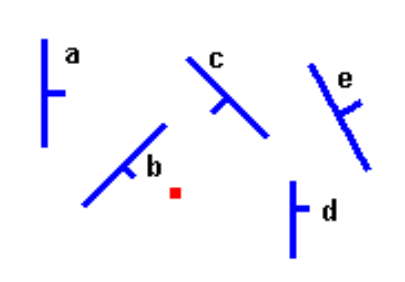
\includegraphics[scale=0.4]{img1}
\end{center}

\tri Схема алгоритма:
\begin{enumerate}
    \item Выбор \emph{сплиттера} среди входных полигонов;
    \item Рассечение набора полигонов на пространство перед сплиттером и за ни;
    \item Вызов алгоритма для каждой из половинок, продолжать пока входной набор полигонов не будет состоять из одного полигона;
\end{enumerate}

\end{frame}





\begin{frame}{BSP дерево: построение}
\footnotesize

\begin{center}
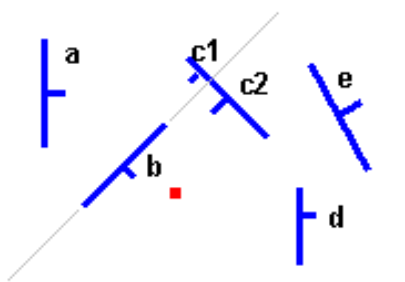
\includegraphics[scale=0.3]{img2}
\end{center}
\tri Выбрав сплиттер, мы можем при помощи алгоритма, использованного при построении CSG-геометрии, поделить остальные полигоны на два множества:
\begin{enumerate}
    \item Те что стоят со стороны нормали сплиттера или коплонарны ему и совпадают с ним нормалью переходят в первое множество;
    \item Те что стоят сзади сплиттера или коплонарны ему и противоположны с ним по нормали переходят во второе множество;
    \item Если полигон пересекается плоскостью сплиттера, то он рассекается.
\end{enumerate}
Полигон сплиттера кладётся в вершину.
\begin{center}
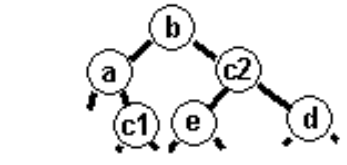
\includegraphics[scale=0.4]{img3}
\end{center}

\end{frame}





\begin{frame}{BSP дерево: построение}
\footnotesize

\begin{center}
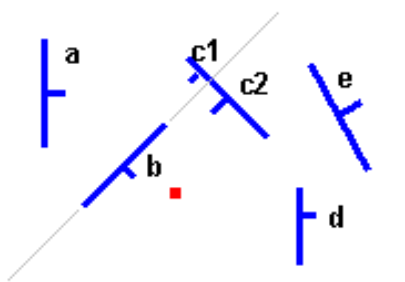
\includegraphics[scale=0.3]{img2}
\end{center}
\tri Выбор сплиттера не случаен. От стратегии выбора зависит размер дерева. Полный перебор вариантов NP-сложен, потому применяют метрические оценки, например стремятся уменьшить разницу между число полигонов перед полигоном и за ним:
\begin{equation}\nonumber
    \min |front - back|.
\end{equation}

\tri Пример:
\begin{center}
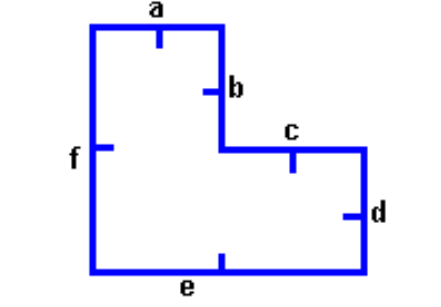
\includegraphics[scale=0.3]{img4}
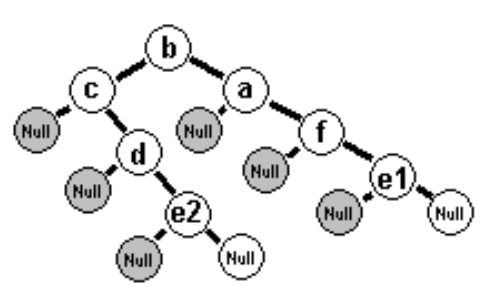
\includegraphics[scale=0.3]{img5}
\end{center}

\end{frame}





\begin{frame}{BSP дерево: отрисовка}
\footnotesize

\tri BSP дерево позволяет сортировать полигоны в порядке удалённости.

\end{frame}





\end{document}















